% Overall architecture of STATOR: every serving process maps the model file
% and the published prefix read-only and writes its own rows to a private
% tail; the GPU of either MIG instance reads all of it in place through the
% host page tables.
\documentclass[border=2pt]{standalone}
% Shared TikZ style of the STATOR design figures. Teal marks shared,
% immutable state; amber marks what one process writes; violet marks a
% second level of sharing; text is regular weight except the panel titles.
\usepackage{newtxtext}
\usepackage{tikz}
\usetikzlibrary{arrows.meta, positioning, fit, calc, patterns, shapes.geometric, decorations.pathreplacing}

\definecolor{panel}{HTML}{F3F4F6}   % a group of components
\definecolor{gpuc}{HTML}{E4E0F6}    % the GPU
\definecolor{ptc}{HTML}{FAF0DC}     % page tables and the SMMU
\definecolor{modelc}{HTML}{CDEBE6}  % the weights
\definecolor{sharedc}{HTML}{7FCBC1} % shared rows, read-only
\definecolor{tailc}{HTML}{F7B955}   % rows of one process, in use
\definecolor{aheadc}{HTML}{FCE6C2}  % populated ahead, or write-protected
\definecolor{copyc}{HTML}{F4BFCB}   % a copied page
\definecolor{segc}{HTML}{B7A9E8}    % the segment of a second ancestor
\definecolor{faultc}{HTML}{E8736A}  % a private copy made by a fault
\definecolor{actc}{HTML}{FDE9C9}    % an operation of the design
\definecolor{roline}{HTML}{14786F}  % read-only mappings
\definecolor{rwline}{HTML}{C5432F}  % writable mappings and faults

\tikzset{
  layer/.style={draw=black!60, fill=panel, line width=0.5pt},
  sub/.style={draw=black!55, line width=0.4pt},
  comp/.style={draw=black!85, fill=white, line width=0.4pt, align=center,
               font=\scriptsize, inner xsep=3pt, inner ysep=1.5pt, minimum height=0.5cm},
  seg/.style={draw=black!65, line width=0.35pt, inner sep=0pt, align=center,
              font=\scriptsize, minimum height=0.4cm},
  free/.style={seg, pattern=north east lines, pattern color=black!40},
  blk/.style={draw=black!65, line width=0.35pt, minimum width=0.42cm, minimum height=0.36cm,
              inner xsep=2pt, inner ysep=0pt, font=\scriptsize},
  hole/.style={blk, pattern=north east lines, pattern color=black!45},
  tag/.style={font=\scriptsize, inner sep=1pt},
  ttl/.style={font=\bfseries\small},
  lbl/.style={font=\scriptsize},
  note/.style={font=\itshape\scriptsize, inner sep=1pt},
  arr/.style={-{Latex[length=1.6mm]}, line width=0.8pt},
  thin/.style={-{Latex[length=1.3mm]}, line width=0.5pt},
  fat/.style={-{Triangle[length=2.2mm,width=3.4mm]}, line width=2.4pt},
  num/.style={circle, fill=black, text=white, font=\bfseries\scriptsize,
              inner sep=0.6pt, minimum size=0.33cm},
}
% A legend entry: a filled square and its name, at (x,y).
\newcommand{\legendfill}[4]{%
  \draw[black!65, line width=0.35pt, fill=#3] (#1,#2) rectangle ++(0.22,0.2);
  \node[tag, anchor=west] at (#1+0.27,#2+0.1) {#4};}
\newcommand{\legendhatch}[3]{%
  \draw[black!65, line width=0.35pt, pattern=north east lines, pattern color=black!45] (#1,#2) rectangle ++(0.22,0.2);
  \node[tag, anchor=west] at (#1+0.27,#2+0.1) {#3};}
% Legend marks for a legend that is one centred line of text:
%   \node[tag] at (x,y) {\lgdfill{sharedc}\,Shared \quad \lgdhatch\,Unbacked};
\newcommand{\lgdfill}[1]{\tikz[baseline=-0.55ex]{\draw[black!65, line width=0.35pt, fill=#1] (0,-0.1) rectangle (0.22,0.1);}}
\newcommand{\lgdhatch}{\tikz[baseline=-0.55ex]{\draw[black!65, line width=0.35pt, pattern=north east lines, pattern color=black!45] (0,-0.1) rectangle (0.22,0.1);}}

\begin{document}
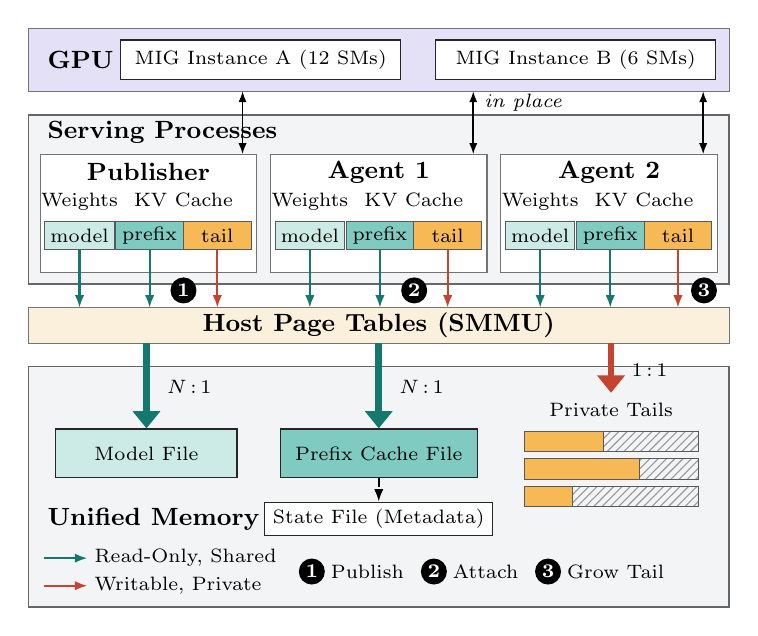
\begin{tikzpicture}[x=1cm, y=1cm]

% ---------------- GPU ----------------
\draw[sub, fill=gpuc] (0,6.55) rectangle (8.9,7.35);
\node[ttl, anchor=west] at (0.12,6.95) {GPU};
\node[comp, minimum width=3.55cm, minimum height=0.5cm] (miga) at (2.95,6.95) {MIG Instance A (12 SMs)};
\node[comp, minimum width=3.55cm, minimum height=0.5cm] (migb) at (6.95,6.95) {MIG Instance B (6 SMs)};

% ---------------- serving processes ----------------
\draw[layer] (0,4.1) rectangle (8.9,6.25);
\node[ttl, anchor=west] at (0.12,6.03) {Serving Processes};
\newcommand{\process}[3]{% x of the left edge, node prefix, name
  \draw[sub, fill=white] (#1,4.25) rectangle (#1+2.75,5.75);
  \node[ttl] at (#1+1.375,5.52) {#3};
  \node[tag, anchor=base] at (#1+0.5,5.08) {Weights};
  \node[tag, anchor=base] at (#1+1.82,5.08) {KV Cache};
  \node[blk, fill=modelc, minimum width=0.86cm] (#2m) at (#1+0.5,4.72) {model};
  \node[blk, fill=sharedc, minimum width=0.86cm] (#2p) at (#1+1.39,4.72) {prefix};
  \node[blk, fill=tailc, minimum width=0.86cm] (#2t) at (#1+2.25,4.72) {tail};
}
\process{0.15}{pub}{Publisher}
\process{3.075}{one}{Agent 1}
\process{6.0}{two}{Agent 2}
\foreach \x in {2.72,5.65,8.57} {
  \draw[{Latex[length=1.4mm]}-{Latex[length=1.4mm]}, line width=0.6pt] (\x,5.75) -- (\x,6.55);
}
\node[note, anchor=west] at (5.75,6.4) {in place};

% ---------------- host page tables ----------------
\draw[sub, fill=ptc] (0,3.35) rectangle (8.9,3.8);
\node[ttl] at (4.45,3.575) {Host Page Tables (SMMU)};
\foreach \p in {pub,one,two} {
  \draw[arr, roline] (\p m.south) -- (\p m.south |- 0,3.8);
  \draw[arr, roline] (\p p.south) -- (\p p.south |- 0,3.8);
  \draw[arr, rwline]  (\p t.south) -- (\p t.south |- 0,3.8);
}
\node[num] at (1.97,4.02) {1};
\node[num] at (4.9,4.02) {2};
\node[num] at (8.58,4.02) {3};

% ---------------- unified memory ----------------
\draw[layer] (0,0) rectangle (8.9,3.05);
\node[ttl, anchor=west] at (0.12,1.12) {Unified Memory};
\node[comp, fill=modelc, minimum width=2.3cm, minimum height=0.62cm] (mfile) at (1.5,1.95) {Model File};
\node[comp, fill=sharedc, minimum width=2.5cm, minimum height=0.62cm] (pfile) at (4.45,1.95) {Prefix Cache File};
\node[comp, minimum width=2.5cm, minimum height=0.42cm] (sfile) at (4.45,1.12) {State File (Metadata)};
\draw[arr, densely dashed] (pfile.south) -- (sfile.north);
\node[tag] at (7.4,2.5) {Private Tails};
\foreach \y/\u in {2.1/1.0,1.75/1.45,1.4/0.6} {
  \node[seg, fill=tailc, minimum width=\u cm, minimum height=0.26cm, anchor=west] at (6.3,\y) {};
  \node[free, minimum width=2.2cm-\u cm, minimum height=0.26cm, anchor=west] at (6.3+\u,\y) {};
}
\draw[fat, roline] (1.5,3.35) -- (mfile.north);
\draw[fat, roline] (4.45,3.35) -- (pfile.north);
\draw[fat, rwline]  (7.4,3.35) -- (7.4,2.72);
\node[tag, anchor=west] at (1.72,2.8) {$N$\,:\,1};
\node[tag, anchor=west] at (4.67,2.8) {$N$\,:\,1};
\node[tag, anchor=west] at (7.62,3.0) {1\,:\,1};

% ---------------- legend ----------------
\draw[arr, roline] (0.2,0.62) -- (0.75,0.62);
\node[tag, anchor=west] at (0.8,0.62) {Read-Only, Shared};
\draw[arr, rwline] (0.2,0.27) -- (0.75,0.27);
\node[tag, anchor=west] at (0.8,0.27) {Writable, Private};
\node[num] at (3.6,0.45) {1};
\node[tag, anchor=west] at (3.8,0.45) {Publish};
\node[num] at (5.15,0.45) {2};
\node[tag, anchor=west] at (5.35,0.45) {Attach};
\node[num] at (6.6,0.45) {3};
\node[tag, anchor=west] at (6.8,0.45) {Grow Tail};

\end{tikzpicture}
\end{document}
